\chapter{Reusing Classes}

%\section{Inheritance revisited}

When we first looked at inheritance in Chapter~\ref{eights}, our purpose was to avoid duplicating code.
We noticed that ``decks of cards'' and ``hands of cards'' had common functionality, and we designed a \java{CardCollection} class to provide it.
This design technique is known as {\bf generalization}.
By generalizing the code, we were able to reuse it in the \java{Deck} and \java{Hand} classes.

In Chapter~\ref{conway}, we looked at inheritance from a different point of view.
When designing \java{GridCanvas} to represent a grid of cells, we extended \java{Canvas} and overrode its \java{paint} and \java{update} methods.
This design technique is known as {\bf specialization}.
By specializing the code already provided by \java{Canvas}, we were able to draw grids on the screen with very little effort.

Notice that we didn't write the code for \java{Canvas}; it's part of the Java Library.
But we were able to extend it for our own purposes.
In fact, the \java{Canvas} class was specifically designed to be extended.

For this chapter, we'll explore the ideas of specialization and reuse more fully.
We'll continue to develop graphical simulations as a running example, but this time with varying shapes and colors!


\section{Polygon Objects}

The word polygon means ``many angles''; the most basic examples of polygons are triangles (3 angles), rectangles (4 angles), pentagons (5 angles), and so forth.
Polygons are an important part of computer graphics, because they are used to compose more complex images.

Java provides a \java{Polygon} class (in \java{java.awt}) that is relatively straightforward to use.
The following code creates the triangle shown in Figure~\ref{fig:triangle}:

\begin{code}
Polygon p = new Polygon();
p.addPoint(57, 110);
p.addPoint(100, 35);
p.addPoint(143, 110);
\end{code}

\begin{figure}[!ht]
\begin{center}
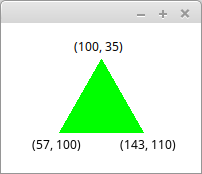
\includegraphics[scale=1]{figs/triangle.png}
\caption{A polygon with three points.}
\label{fig:triangle}
\end{center}
\end{figure}

Internally, \java{Polygon} objects have three attributes:

\begin{itemize}
\item \java{public int npoints;} {\tt ~~~} \java{// total number of points}
\item \java{public int[] xpoints;} {\tt ~} \java{// array of X coordinates}
\item \java{public int[] ypoints;} {\tt ~} \java{// array of Y coordinates}
\end{itemize}

%The \java{npoints} attribute makes it possible to add points to the polygon one at a time.
When a \java{Polygon} is created, \java{npoints} is 0 and the two arrays are initialized with length 4.
As points are added, \java{npoints} is incremented.
If \java{npoints} exceeds the length of the arrays, larger arrays are are created on the fly, and all the data is copied from the previous arrays.

The \java{Polygon} class provides many useful methods like \java{contains}, \java{intersects}, and \java{translate}.
However, it doesn't provide any methods for displaying the polygon like \java{draw} or \java{toString}.


\section{Adding Color}

Specialization is useful for adding new features to an existing class, especially when you can't (or don't want to) change its design.
For example, we can specialize the \java{Polygon} class by adding a \java{Color} attribute and implementing a \java{draw} method:

\begin{code}
public class ColorPolygon extends Polygon {
    public Color color;

    public ColorPolygon() {
        super();
        color = Color.GRAY;
    }
    
    public void draw(Graphics g) {
        g.setColor(color);
        g.fillPolygon(this);
    }
}
\end{code}

As a reminder, constructors are not inherited when you extend a class.
If you don't define a constructor, the compiler will generate one for you that does nothing.
The constructor for \java{ColorPolygon} uses the \java{super} keyword to invoke the constructor for \java{Polygon}.
It then initializes the color to \java{GRAY}.

\java{ColorPolygon} has the same attributes and methods that \java{Polygon} has, in addition to \java{color} and \java{draw}.
You can use \java{addPoint} as before, or you can directly access \java{npoints}, \java{xpoints}, and \java{ypoints} (since they are \java{public}).
You can also use methods like \java{contains}, \java{intersects}, and \java{translate}.

The following code creates the triangle shown in Figure~\ref{fig:triangle} and sets its color to \java{GREEN}:

\begin{code}
ColorPolygon p = new ColorPolygon();
p.addPoint(57, 110);
p.addPoint(100, 35);
p.addPoint(143, 110);
p.color = Color.GREEN;
\end{code}


\section{Regular Polygons}

The \java{Polygon} class provides only two constructors: one that creates an empty polygon, and one that copies values into \java{xpoints}, \java{ypoints}, and \java{npoints}.
Create polygons with many sides can be very tedious.
It would be nice if we could just ask for 20-sided polygon of size 50, for example, without having to specify all the coordinates.
We can extend ColorPolygon to do just that.
